\documentclass{ifacconf}

\usepackage[numbers,sort]{natbib}   % you should have natbib.sty
\usepackage{graphicx}          % Include this line if your 
                               % document contains figures,
%\usepackage[dvips]{epsfig}    % or this line, depending on which
                               % you prefer.
% predefined environments
%\begin{thm} ... \end{thm}		% Theorem
%\begin{lem} ... \end{lem}		% Lemma
%\begin{claim} ... \end{claim}	% Claim
%\begin{conj} ... \end{conj}	% Conjecture
%\begin{cor} ... \end{cor}		% Corollary
%\begin{fact} ... \end{fact}	% Fact
%\begin{hypo} ... \end{hypo}	% Hypothesis
%\begin{prop} ... \end{prop}	% Proposition
%\begin{crit} ... \end{crit}	% Criterion
\newcommand{\secref}[1]{Section~\ref{#1}}	

\begin{document}

\begin{frontmatter}

\title{Toward Random Number Generation on Commodity Hardware\thanksref{footnoteinfo}} % Title, preferably not more than 10 words.

\thanks[footnoteinfo]{This paper was written as part of the course PPPRS at Aalborg University 2012-2013. Citation of this paper is not allowed.}

\author[First]{Alex Bondo Andersen} 

\address[First]{Department of Computer Science �- Selma Lagerl�fs Vej 300 -� DK-9220 Aalborg East -- Email: aban09@student.aau.dk}   
          
%\begin{keyword}                           % Five to ten keywords,  
%Cicero; Catiline; orations.               % chosen from the IFAC 
%\end{keyword}                             % keyword list or with the 
                                          % help of the Automatica 
                                          % keyword wizard


\begin{abstract}                          % Abstract of not more than 250 words.
In this paper research is conducted toward a much faster random number generator which can run on commodity hardware without need for extra devices.
The random number generator, Parallel Memory Writer, presented here uses several physical execution units to generate random numbers.
A performance test is conducted and used as comparison with both a random number generator and a pseudo-random number generator, showing a significant improvement over the other RNG.
\end{abstract}

\end{frontmatter}

\section{Introduction}
\label{sec:intro}
Random numbers are generated for several different purposes.
Games, gambling, art, cryptography, and Monte Carlo methods to name a few~\citep{Stojanovski01chaos-basedrandom}.
These areas have different requirements for their random number generator and each application has a further specific set of requirements for its generator.
Pseudo-random number generators (PRNGs) rely on a sequence of ``seemingly'' random numbers initialized by a seed.
This sequence will repeat itself after a given \emph{period}, albeit this is often large -- the Mersenne Twister was implemented in 1998 with a period of $2^{19937}-1$~\citep{Matsumoto98}.
The period indicates the size of the sequence of numbers -- the PRNG will simply repeat the sequence if the required amount of pseudo-random numbers is greater than the period.
These are usually very fast, but are not truly random and therefore not applicable for security oriented applications, such as cryptography.

An alternative is to use physical conditions as a source of entropy in order to make a true random number generator (RNG).
Solutions in this direction include usage of photoevents~\citep{Martino91}, generation (and reading) of random noise~\citep{Holman97}, and reading atmospheric noise~\citep{random.org}.
These methods for obtaining true random numbers require extra hardware to function.
Furthermore, an attacker might be able to place a sensor near the one used by the RNG and thus have higher probability of guessing the generated numbers.
This is, however, only speculation.
Web-services, such as www.random.org~\citep{random.org}, has the required hardware to generate true random numbers which are accessible through their service.
This, of course, requires a connection to the web-service and trust in its authenticity.

Another alternative is to use events internal in the hardware connected the computer where the random numbers are to be generated.
The Linux device \devrandom{}~\citep{devrandom} uses keyboard, mouse, and network events to generate highly unpredictable, and thus random, numbers.
To accomplish this external devices must be connected to the computer, albeit very common external devices.

The approach that I am taking to generate random numbers requires no external devices, no network connectivity, and produces random numbers of cryptographic quality.
This approach utilizes different physical cores in the processor to generator numbers which for practical purposes are random.
Such an approach is, to the best of my knowledge, novel.
Parallel computing has been used in random number generators, but primarily for speedup~\citep{parallelRand}, not to increase the unpredictability.
I call my approach \emph{Parallel Memory Writer} (PMW).

The remainder of the paper is divided into four sections.
First, \secref{sec:method} describes the details of how the random numbers are generated.
\secref{sec:result} shows the results from performance tests of PMW.
These results are discussed and evaluated in \secref{sec:discussion}.
Finally a conclusion is drawn in \secref{sec:conclusion} together with future research directions.

%Something about randomness is in the eye of the beholder, but we choose to test through dieharder or what ever
\section{Method}
\label{sec:method}
To generate highly unpredictable numbers I use the fact that predicting the order of action of different threads of execution can be extremely difficult even when the actual hardware is available.
Figure~\ref{fig:TrueRand} illustrates two threads of execution writing different values to the same bit in memory.
When this bit in memory, $Mem_0$, is read at a some point in time, it is not possible to know in advance which value it contains without direct access to the internal hardware of the computer.

\begin{figure}
	\centering
		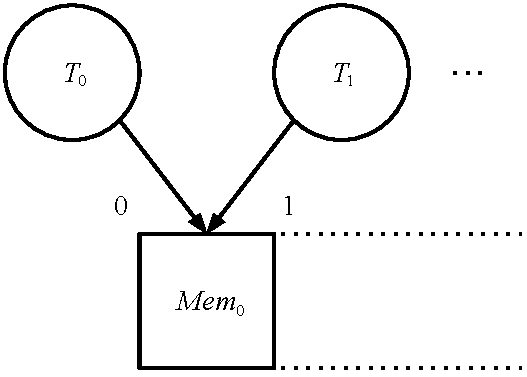
\includegraphics[width=0.5\columnwidth]{image/TrueRand.pdf}
	\caption{Two threads of execution writing to the same bit of memory.}
	\label{fig:TrueRand}
\end{figure}

Now that we can construct a single unpredictable bit, the challenge is to expand it to generate larger sequences of memory with unpredictable value.
To accomplish this the first step is simply to add more threads of execution, two to each bit of memory.
Secondly we add a bitmap which indicates whether or not a bit has been touched.
A bit is \emph{touched} when one of the two threads writing to it has actually written something to it.
E.g. $Bitmap_0=0$ until either $T_0$ or $T_1$ has written to $Mem_0$.
When a user of the generator requests a random number, he cannot be served until all the bits in $Mem$ has been touched, i.e. $Bitmap$ contain only 1's.
This technicality ensures that binary structure of each generated number has no association to the previously generated number.
%This technicality ensures that the generator will work even when the random memory block to be generated contains more than half as many bits as there are cores in the processor -- each bit in $Mem$ requires two threads.
If a user is very eager to get many random numbers, two requests might be received before some pair of $T$s have had their chance to write to their associated $Mem_i$ and thus generating a number with the same value in the $i$th binary digit as the previously generated number.

A considered alternative was to require a predefined time to elapse before the user is served with a number.
This was rejected due to two factors;
First, different computers, operating systems (OS), and implementations might behave slightly differently and hence it would require the time to be quite high or risk compromising the quality of the generated random numbers.
Secondly, I aim to allow PMW to run on commodity hardware which means that the workload of the computer can possible change quite dramatic as the user uses his computer for other purposes while random numbers are being generated -- again forcing the a pessimistic choice in time limit.
It might be noted that the fact that the user is using his computer might actually increase the entropy much the same way as for the Linux device \devrandom{}.
PMW uses this entropy indirectly compared to \devrandom{}.
The thread scheduler of the OS will generally try to achieve a fair amount of execution time for each thread.
Since the user of the computer is starting and stopping threads, the scheduler will move the execution of threads (the PMW writing threads in particular) around both in time and physical computation units (cores).
E.g. if the user starts a new process the execution of a PMW writing thread might be delayed, thus potentially increase the entropy since this delay is very difficult to predict in advance.

It is important that for all $i\in\left[0..\left|Mem\right|-1\right]:$ $T_{2i}$ and $T_{2i+1}$ are executed on different physical cores.
Otherwise, a pattern in the execution of the two threads might give itself away, provided a sufficient number of random numbers are generated.

To test PMW a predefined number of random samples of constant size are requested and the time which it takes to generate these bytes logged.
The throughput of the generator is calculated as the number of samples per time unit.
This throughput is used as comparison to other RNGs.
\section{Result}
\label{sec:result}
To test the performance of RMW between 1 to 10,000,000 bytes are generated in different test cases.
PMW is implemented in C++ and uses the standard library of C++ along with Boost C++ Libraries~\citep{boost}.
The test cases are run on an Intel Core i7 2.93 GHz with 8 GB RAM operated by Windows 7 64 bit SP 1.

The results of the performance tests are shown in Table~\ref{tab:tests}
For comparison the standard library random number generator in C has a throughput of $\approx 7500$ samples/ms and \texttt{/dev/random} has a throughput $<0.001$ sample/ms $=1$ sample/s.
Note that \texttt{/dev/random} is run on another computer running Ubuntu OS, with an initially empty pool of entropy.
This computer is a server and hence has no directly connected keyboard or mouse.

\begin{table}
	\centering
		\begin{tabular}{|l|l|l|}
			\hline
			Samples&Time (ms)&Throughput (samples/ms)\\
			\hline
			1&5&0.20\\
			\hline
			10&18&0.56\\
			\hline
			100&38&2.6\\
			\hline
			1,000&90&11\\
			\hline
			10,000&740&14\\
			\hline
			100,000&7202&14\\
			\hline
			1,000,000&83314&12\\
			\hline
			10,000,000&853632&12\\
			\hline
		\end{tabular}
	\caption{Results from performance tests}
	\label{tab:tests}
\end{table}

In combination with the performance tests the generated numbers are logged and a distribution can be seen in Figure~\ref{fig:distribution}.
The bytes are represented by their decimal values.

\begin{figure}
	\centering
		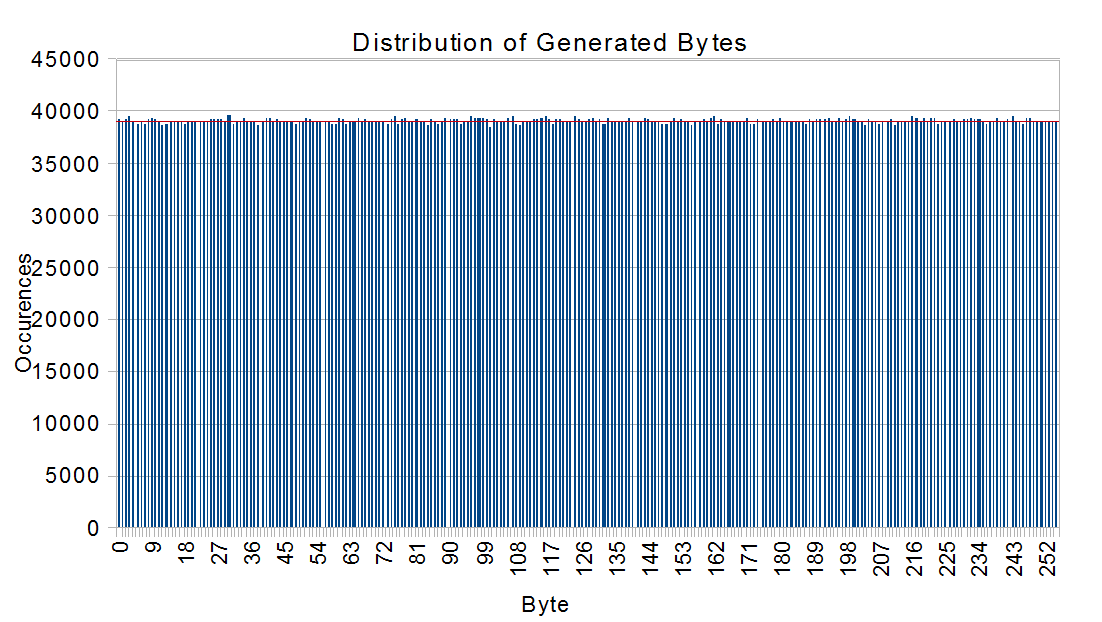
\includegraphics[width=\columnwidth]{image/distribution.png}
	\caption{Distribution of $10^7$ random bytes.}
	\label{fig:distribution}
\end{figure}

\section{Discussion}
\label{sec:discussion}
As shown in Figure~\ref{tab:tests} the throughput increases as more random numbers (bytes) are requested.
This is dues to the startup cost for initializing the generator and auxiliary objects -- such as the timer itself -- before generation can start.
It is peculiar that the throughput of random numbers actually drops when the number of generated bytes is over $10^5$.
The reason is unknown, but fluctuations in workload of the test computer is a possible explanation, as the test computer is a simple desktop computer running other applications and services along with PMW.

As shown the PMW is very slow compared to a standard library implementation of a PNRG.
This is the trade-off that must be considered when deciding between an actual RNG and a PRNG.
On the other hand it is very fast compared to other true RNGs.
\devrandom{} can take up to several minutes just to generate a few hundred bytes if the pool of entropy is empty.
This means that PMW has a throughput several orders of magnitude higher that \devrandom{}.
It should be kept in mind that \devrandom{} is run on different hardware than PMW, with slower CPU and less memory.
This, however, should not affect \devrandom{}, since the bottleneck is neither computation time nor memory, but rather sources of entropy.

The distribution of random bytes in Figure~\ref{fig:distribution} shows that no byte seem to appear much more often than any other.
This means that PMW exhibit equi-distribution, which is generally a desirable property of an RNG since other distributions (such as normal distribution) can be constructed based on it.
Furthermore, it does not seem that there is a noticeable structure in which bytes are a little more represented than others.
This is desirable since it means that a potential attacker will have difficulty in guessing what is to be generated even if he has access to previously generated numbers.
\section{Conclusion \& Future Work}
\label{sec:conclusion}
An RNG called Parallel Memory Writer is created and presented in this paper.
It requires no extra hardware devices, no Internet connectivity and yet provides unpredictability of the numbers generated.
It accomplishes this by utilizing several physical execution cores which are found in most modern processors.
Although slower than PNRGs it is several orders of magnitude faster than other common RNGs.

As this paper presents work toward random number generation there are without a doubt several interesting direction which research might expand. I here present those which I believe are the most essential.
Future work on PMW is to test it with a test battery for random number generators such as \emph{Dieharder}~\citep{dieharder}.
The results could then be compared with those of common PRNGs such as the Mersenne Twister.
Another interesting research direction could be to combine PMW with a seeded PRNG such that a random seed is generated by PMW and used to produce random numbers much faster through the PNRG, which might be reseeded periodically.
%\begin{ack}                               % Place acknowledgements

\end{ack}

%

\bibliography{bib}           % and a bib file to produce the 
%\bibliography{autosam}
                                 % bibliography (preferred). The
                                 % correct style is generated by
                                 % Elsevier at the time of printing.



%\appendix
\end{document}